\documentclass[titlepage]{article}
\usepackage{listings}
\usepackage{hyperref}

\lstset{basicstyle=\footnotesize\ttfamily,breaklines=true}

\usepackage{tikz}
\usetikzlibrary{arrows}

\begin{document}
\title{Trains Control 1}
\author{Justin McGirr (\#20413625), Peter Raboud (\#20437716)}
\maketitle

\section{Instructions}
\subsection{Installation}\label{installation}

Simply run \texttt{make ENV=ts7200 install}. This will place the
compiled kernel in \texttt{/u/cs452/tftp/ARM/\$(USER)/k.elf} (where
\texttt{\$(USER)} is whatever your username is on the computer which you
are compiling it). You can then load this kernel from redboot using
\texttt{load -b 0x00218000 -h 10.15.167.5 "ARM/\$(USER)/k.elf"}. At this
stage, the kernel doesn't do much that is particularly interesting,
there is no shell or other interactive elements, it simply runs the code
which it was given.

\subsection{Emulator}\label{emulator}

You can run the OS on an emulated arm CPU via
\texttt{make ENV=qemu qemu-run}. In order for this to complete
successfully, you will need:

\begin{itemize}
\itemsep1pt\parskip0pt\parsep0pt
\item
  A local install of QEMU
\item
  A local install of an arm-none-eabi toolchain
\end{itemize}

\subsection{Tests}\label{tests}

The provided kernel has some basic tests, which you can run with
\texttt{make ENV=qemu test}. (this depends on the emulator, above).

\subsection{Debugging}\label{debugging}

If something goes wrong and you want to investigate deeper, you can run
\texttt{make ENV=qemu qemu-start} in one terminal (this starts qemu in a
suspended state), and then \texttt{make ENV=qemu qemu-debug} in another.
You can then set breakpoints, step, inspect memory, etc- anything you
can normally do with gdb.

\subsection{Special Instructions}\label{special-instructions}

Before running the program on the TS7200, it is necessary to reset both
the TS7200 and the train controller, to avoid messy state left behind by
previous runs. In particular, this has been known to cause bugs with the
sensor reads, where garbage data left in the UART is picked up, and
misinterpreted.

\subsection{Useful links:}\label{useful-links}

\subsubsection{General}\label{general}

\begin{itemize}
\itemsep1pt\parskip0pt\parsep0pt
\item
  \href{http://www.cgl.uwaterloo.ca/~wmcowan/teaching/cs452/pdf/arm-architecture.pdf}{ARMv4
  Manual}
\item
  \href{http://ascii-table.com/ansi-escape-sequences.php}{Terminal
  escape sequences}
\end{itemize}

\subsubsection{TS7200 hardware}\label{ts7200-hardware}

\begin{itemize}
\itemsep1pt\parskip0pt\parsep0pt
\item
  \href{http://www.cgl.uwaterloo.ca/~wmcowan/teaching/cs452/pdf/ts-7200-manual.pdf}{TS7200
  Manual}
\item
  \href{http://www.cgl.uwaterloo.ca/~wmcowan/teaching/cs452/pdf/ep93xx-user-guide.pdf}{Cirrus
  EP9302 Manual}
\item
  \href{http://www.cgl.uwaterloo.ca/~wmcowan/teaching/cs452/pdf/icu-pl190.pdf}{Interrupt
  controller manual}
\end{itemize}

\subsubsection{VersatilePB hardware emulated by
QEMU}\label{versatilepb-hardware-emulated-by-qemu}

\begin{itemize}
\itemsep1pt\parskip0pt\parsep0pt
\item
  \href{http://infocenter.arm.com/help/topic/com.arm.doc.dui0224i/DUI0224I_realview_platform_baseboard_for_arm926ej_s_ug.pdf}{SOC
  manual}
\item
  \href{http://infocenter.arm.com/help/topic/com.arm.doc.ddi0271d/DDI0271.pdf}{Timer
  manual}
\item
  \href{http://infocenter.arm.com/help/topic/com.arm.doc.ddi0181e/DDI0181.pdf}{Interrupt
  controller manual} (Same as the TS7200 hardware)
\item
  \href{http://infocenter.arm.com/help/topic/com.arm.doc.ddi0183f/DDI0183.pdf}{UART
  Manual}
\end{itemize}


\section{Design Decisions}
% trainsrv
% - landmark + dead reckoning
% - basic sensor attribution
% - traversal of track, helper methods
% train alert srv

% acceleration profile
% initial v0 -> v1 way to get stopping distance (failed because can't run the
% train at low speed)
% partial deceleration method
% train selfie data, and conclusions
% bisection to find the stopping distance

% talk about nested functions?
% talk about new compiler?

\subsection{Overview}

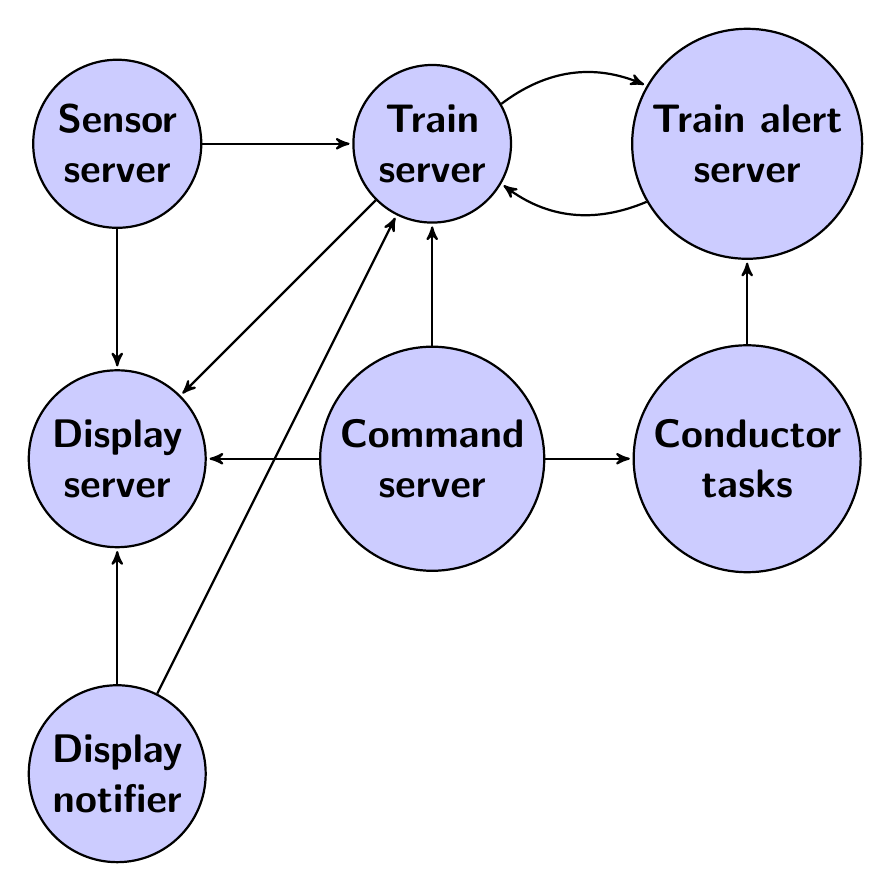
\begin{tikzpicture}[->,>=stealth',shorten >=1pt,auto,node distance=4cm,
  thick,main node/.style={circle,fill=blue!20,draw,font=\sffamily\Large\bfseries}]

  \node[main node] (d) [align=center]{Display \\ server};
  \node[main node] (dn) [align=center, below of=d]{Display \\ notifier};
  \node[main node] (c) [align=center, right of=d] {Command \\ server};
  \node[main node] (t) [align=center, above of=c] {Train \\ server};
  \node[main node] (ta) [align=center, right of=t] {Train alert \\ server};
  \node[main node] (s) [align=center, left of=t] {Sensor \\ server};
  \node[main node] (e) [align=center, right of=c] {Conductor \\ tasks};

  \path[every node/.style={font=\sffamily\small}]
    (dn) edge node {} (d)
         edge node {} (t)
    (t) edge [bend left] node {} (ta)
        edge node {} (d)
    (ta) edge [bend left] node {} (t)
    (c) edge node {} (t)
        edge node {} (d)
        edge node {} (e)
    (e) edge node {} (ta)
    (s) edge node {} (t)
        edge node {} (d)
    ;
    % (2) edge node [right] {0.4} (1)
    %     edge node {0.3} (4)
    %     edge [loop left] node {0.4} (2)
    %     edge [bend right] node[left] {0.1} (3)
    % (3) edge node [right] {0.8} (2)
    %     edge [bend right] node[right] {0.2} (4)
    % (4) edge node [left] {0.2} (3)
    %     edge [loop right] node {0.6} (4)
    %     edge [bend right] node[right] {0.2} (1);
\end{tikzpicture}

\subsection{Train Server}
To help manage the position of the trains, we changed the structure of the
tasks somewhat.
The train server was significantly altered.
Its original purpose was to be a simple server to interact with the track,
and was only a separate task so that we could globally keep track of the
speed a train is travelling at, and the orientation of the switches.

Now, this role has been significantly expanded into keeping track of the
positions of the trains, and inferring them based on incoming sensor data.
The train server keeps track of the last sensor a particular train hit.
Currently, we don't have proper sensor attribution, so we can only support
one train on track at once, but most of the train server is not written with
this assumption.
Since it's assumed that there is only one train on the track, and that
it is responsible for any sensor that is tripped.
Whenever a sensor is tripped, the assumed position of the train snaps to that
location.
This does not account for spurious sensor reads, other than ignoring
sensors that are continuously tripped.
(This was done since the sensor data from track B would otherwise be unusable.)

We infer the velocity of the train from these sensor reads, since we can
find the distance between this sensor, and the last one, and the time between
the reads, and calculate the velocity the train must have been travelling at.
This assumes that the train travels at a constant speed, which is acceptably
close to the truth for our purposes.
If the new sensor read means that the train seems to have travelled past
another sensor without tripping it, we are tolerant of this.
The distance travelled is considered to be the sum of the lengths of track
between each pair of sensors.
If more than one sensor would have needed to be missed, we still consider the
train to now be at this location, but we don't use this data to estimate
a velocity, since it's likely that something strange happened, and that
the data is not valid.
We incorporate the calculated velocity from each interval of track by computing
a new estimate of the velocity from the old estimate $v_e$, and the measured
velocity $v_a$.
We use the heurestic $v_e' = (1 - \alpha) v_e + \alpha v_a$, for $\alpha = 0.1$.

We also record how far off our previous estimate was, by computing where
we thought the train was at the moment that it tripped the sensor.
This discrepancy is displayed on the screen, and can be used as a measure of
how well-calibrated the train is.

Based on the estimated velocity, last sensor tripped, and time the last sensor
was tripped, we can estimate the current position of the train.
We also have the notion of "reanchoring" the trains - updating the last
known position to the currently estimated position.
Whenever we change the speed of a train, we reanchor that train.
When the orientation of a turnout is changed, we reanchor all trains.
This simplifies the computation that needs to be done to project the position
of the train, since it allows us to assume that the speed of the train and
orientation of the turnouts hasn't changed during the period we want to predict
the motion of the train.
By making these assumptions, as well as the assumption that the trains accelerate
instantaenously, we can calculate the distance traveled since the last position
a train was anchored at as simply the velocity of that train multiplied by
the elapsed time.

\subsection{Train alert server}
An operation that turns out to be useful when writing high-level train control
routines is to wait until the train is at a particular position.
We therefore created a train alert server to allow tasks to wait until a train
has arrived at a particular position.
The interface for the train alert server is
\texttt{int train\_alert\_at(int train\_id, struct position position)}.
The call blocks until the given train is estimated to have passed that position
on the track.
The function returns with the time at which the train passed that position
(time is measured in ticks since the startup of the clockserver).

The train server pushes notifications to the train alert server when
it detects that a train has hit a sensor.
The train alert server has a list of tasks which are waiting on a train
to be in a particular position.
If the sensor data tells the train alert server that this is the last
sensor the train will hit before arriving at the point of interest,
it starts a timer.
This timer waits for the estimated amount of time needed for the train
to travel to the POI, given it's current velocity and the orientation
of the turnouts.
It then wakes up, and signals the alert server that the waiting task can
now be woken up.

If the speed of the train or the orientation of the turnouts is changed
during this wait time, this needs to be detected.
Each await request maintains a nonce.
When a timeout is started, the worker task doing the timeout is given
that nonce.
If the orientation of the turnouts or speed of the train is changed,
the nonce is incremented by one, and a new timeout is begun.
If the nonce doesn't match the nonce that the timeout has, then something
must have changed during the timeout, so the timeout is simply ignored.

\section{Source Code}
The source code is hosted on git, at \url{git.uwaterloo.ca/pgraboud/cs452-kernel}.
The version we wish to submit is the \texttt{tc1} tag, specifically
the commit:
\input{|"git rev-parse HEAD | ./../verbatim"}
\end{document}
